\usetikzlibrary{arrows,automata}

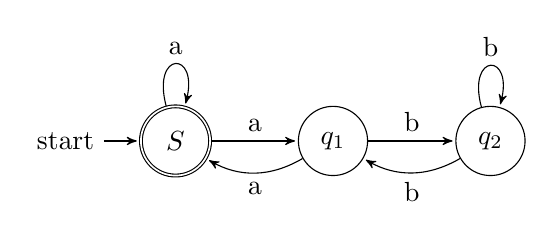
\begin{tikzpicture}[>=stealth',shorten >=1pt,auto,node distance=2cm]
  \node[initial,state,accepting] (S)      {$S$};
  \node[state]         (q1) [right of=S]  {$q_1$};
  \node[state]         (q2) [right of=q1] {$q_2$};


  \path[->] (S)  edge [loop above] node {a} (S)
             edge              node {a} (q1)
        (q1) edge [bend left]  node {a} (S)
             edge              node {b} (q2)
        (q2) edge [loop above] node {b} (q2)
             edge [bend left]  node {b} (q1);
\end{tikzpicture}
